\documentclass{article}
\PassOptionsToPackage{numbers,compress}{natbib}
\usepackage[final]{neurips_2023}
\usepackage[utf8]{inputenc}
\usepackage[T1]{fontenc}
\usepackage{hyperref}
\usepackage{url}
\usepackage{booktabs}
\usepackage{amsfonts,amsmath,amssymb}
\usepackage{nicefrac}
\usepackage{microtype}
\usepackage{graphicx}
\usepackage{xcolor}
\graphicspath{{../figs/}}

\title{Does Superposition Need More Bits? \\ A Preregistered Test of a Precision--Capacity Law}

\author{%
  Lakshya \\
  \texttt{lakyvasu22@gmail.com}
}

\begin{document}
\maketitle

\begin{abstract}
%ABSTRACT%
\end{abstract}

\section{Introduction}

Neural networks represent more features than they have dimensions by assigning them non-orthogonal
directions---\emph{superposition}~\cite{elhage2022toy}. Every quantitative account of superposition to date
assumes infinite-precision weights. Yet a direction is only as resolvable as the numerical grid it is stored
on, which suggests a simple and testable idea: \emph{a layer that superposes more features per dimension should
need more bits}. If true, this would convert a mechanistic quantity (features per dimension, $F$) into an
engineering one (a critical bit-width, $b_{\mathrm{crit}}$), and it would give a first-principles reason for the
empirical folklore that outlier-heavy layers quantize badly~\cite{dettmers2022,xiao2023,lin2024awq}.

We preregistered a closed-form version of this hypothesis, $b_{\mathrm{crit}} = 1 + \log_2\!\big(1 + \kappa\sqrt{F/3}\big)$
with $\kappa = \max|W|/\mathrm{rms}(W)$ measured, i.e.\ half a bit per doubling of $F$, together with decision bands,
controls and a real-model bridge (all in \texttt{PREDICTIONS.md}, committed before any experiment ran). We then tested
it in toy models of superposition (TMS) trained with quantization-aware fake quantization across a $14\times$ range of
$F$, under post-training quantization of the same models, against five non-quantization damage families, and
per weight matrix in GPT-2 small.

\paragraph{Findings.} (i)~The preregistered law is \textbf{rejected}: the critical bit-width is flat in
$F$ (slope %E1SLOPE% bits per doubling, 95\% CI %E1CI%; predicted $0.5$), at $\approx$%BCRIT% bits for round-to-nearest
quantization across $F\in[4,%FMAX%]$, both under quantization-aware training and post-training quantization.
(ii)~The threshold is instead set by a \emph{universal tolerance to relative weight perturbation}: every noise-like
damage family (RTN, dithered, stochastic rounding, per-channel, Gaussian) costs 5\% of the represented features'
explained variance at the same relative perturbation $\sigma_{\mathrm{rel}} = \lVert D(W)-W\rVert_F/\lVert W\rVert_F
\approx %SIGCRIT%$, independent of $F$; structured damage (rank truncation, feature dropout) behaves differently.
(iii)~A corrected derivation explains the null: at $F\gg1$ the interference added by quantization must be compared
with the interference the model already lives with, and $F$ cancels; what survives is the outlier ratio of the
\emph{live} weights, $\kappa_{\mathrm{live}}$, which predicts the measured $b_{\mathrm{crit}}$ to within
$0.2$ bits with no free parameter. (iv)~In GPT-2 small, per-matrix noise thresholds %LMSUMMARY%.
A negative result on a plausible, preregistered idea, with the mechanism that replaces it, is the contribution.


\section{Setup and the preregistered law}

\paragraph{Model.} We use the standard tied-weight TMS~\cite{elhage2022toy}: $x\in\mathbb{R}^n$ with feature $i$
active with probability $p$ and value $\sim U[0,1]$ when active; $h = Wx$ with $W\in\mathbb{R}^{m\times n}$, $m<n$;
$\hat x = \mathrm{ReLU}(W^\top h + b)$; loss $\mathcal{L} = \mathbb{E}\sum_i I_i (x_i-\hat x_i)^2$ with uniform
importance $I_i=1$ in the main sweep. Writing $W_i$ for column $i$,
$\hat x_i = \mathrm{ReLU}(\lVert W_i\rVert^2 x_i + \sum_{j\ne i}(W_i^{\top}W_j)x_j + b_i)$, so the second term is the
interference that superposition costs. Per feature we measure $\nu_i = \mathbb{E}(x_i-\hat x_i)^2$ against the best
constant predictor $\nu_i^0 = p/3 - p^2/4$ and report $\rho_i = 1-\nu_i/\nu_i^0$; a feature is \emph{live} if
$\lVert W_i\rVert\ge 0.5$ (column norms are bimodal, $\approx1$ or $\approx0$). The superposition ratio is
$F = k_{\mathrm{fp32}}/m$ with $k_{\mathrm{fp32}}$ the number of live columns of the fp32 model.

\paragraph{Quantizer.} Per-tensor symmetric round-to-nearest (RTN) with $q_{\max}=2^{b-1}-1$ levels per sign and
step $\Delta=\max|W|/q_{\max}$, applied to $W$ once and used in both directions (tied weights), trained through a
straight-through estimator (QAT). We also use the same quantizer post-training (PTQ) on converged fp32 models,
plus dithered ($\Delta\,\mathrm{round}((W-u)/\Delta)+u$, fixed per-element $u\sim U[0,\Delta)$), stochastic-rounding
and per-channel variants. The residual $\varepsilon=Q(W)-W$ has $\sigma_\varepsilon\approx\Delta/\sqrt{12}$ and we
always \emph{measure} it.

\paragraph{The preregistered law.} With live columns of unit norm, tied weights double the cross-talk:
for $j\neq i$ the added cross-talk variance is $\approx\sigma_\varepsilon^2(\lVert W_i\rVert^2+\lVert W_j\rVert^2)$;
only live columns interfere (dead columns round to exactly $0$); and $\max|W|=\kappa\,\mathrm{rms}(W)$ grows with
occupancy since $\mathrm{rms}(W)=\sqrt{k/(mn)}$. Summing over the $k$ live interferers, active with probability
$p$ and $\mathbb{E}x^2=\nicefrac13$, the quantization-induced interference variance is
$p\kappa^2k^2/(18\,mn\,q_{\max}^2)$. Setting it equal to the retention threshold $\nu^0/2\approx p/6$ and using
$n\approx k$ gives
\begin{equation}
q_{\max,\mathrm{crit}} = \kappa\sqrt{F/3}\qquad\Longrightarrow\qquad
b_{\mathrm{crit}} = 1+\log_2\!\big(1+\kappa\sqrt{F/3}\big)\;\approx\;\mathrm{const}+\tfrac12\log_2 F .
\label{eq:law}
\end{equation}
The slope $\nicefrac12$ was the preregistered claim (bands: $[0.40,0.60]$ confirmed; $[0.15,0.35]$ a different
exponent; $<0.15$ dead); the intercept is constrained because $\kappa$ is measured, not fitted.

\paragraph{Where it goes wrong (written after the sizing pilot, before the main sweep; \texttt{DEVIATIONS.md}, D2).}
Eq.~\eqref{eq:law} compares the \emph{added} interference with the explainable variance $\nu^0$. But at $F\gg1$ the
fp32 model already carries interference many times $\nu^0$ per feature---the Welch bound gives
$\sum_{j\ne i}(W_i^{\top}W_j)^2\gtrsim F-1$ for unit columns---and survives it through the ReLU with a strongly
negative bias ($b_i\approx-0.5$ to $-0.65$ in our fp32 models). The loss responds to the added cross-talk
\emph{relative to the existing} cross-talk: per pair, added $\approx2\sigma_\varepsilon^2$ against existing
$\approx1/m$, i.e.\ a relative increase $2m\sigma_\varepsilon^2 = 2\lVert\varepsilon_i\rVert^2/\lVert W_i\rVert^2$,
which is the squared relative perturbation of each feature direction, $\sigma_{\mathrm{rel}}^2 =
\lVert Q(W)-W\rVert_F^2/\lVert W\rVert_F^2$ (dead columns contribute zero to both). $F$ cancels. Because the residual
lives on the $\ell=k/n$ live columns while $\mathrm{rms}(W)$ is diluted by the dead ones, the RTN residual is
$\sigma_{\mathrm{rel}} = \kappa\sqrt{\ell}/(\sqrt{12}\,q_{\max}) = \kappa_{\mathrm{live}}/(\sqrt{12}\,q_{\max})$
with $\kappa_{\mathrm{live}} = \max|W|/\mathrm{rms}(W_{\mathrm{live}})$, so the corrected prediction is
\begin{equation}
\sigma_{\mathrm{rel,crit}}\ \text{independent of }F,\qquad
b_{\mathrm{crit}} \approx 1+\log_2\!\Big(1+\frac{\kappa_{\mathrm{live}}}{\sqrt{12}\,\sigma_{\mathrm{rel,crit}}}\Big)
= \mathrm{const}+\log_2\kappa_{\mathrm{live}} .
\label{eq:corrected}
\end{equation}
Superposition enters the bit budget only through the outlier ratio of the live weights, not through $F$. The same
argument applies to any perturbation, so noise-like damage families should share one $\sigma_{\mathrm{rel,crit}}$.


\section{Experiments}

All code, the preregistration, dated deviations and results are in the repository. Every model is trained in fp32
on Apple MPS (Adam, lr $10^{-3}$, 200-step warm-up, cosine decay, batch 1024/512, 6000 steps; $\kappa$ plateaus by
step $\sim$4000), evaluated on $\ge$40k fresh samples ($2\times10^5$ at $p=0.002$) with the quantizer active; all arms of
a (config, seed) share the same data stream and evaluation samples, so contrasts are paired.

\textbf{E0 (trust gate).} fp32 replication of the feature-dimensionality ladder at $n=400$, $m=30$, uniform importance:
$D^\star = m/\sum_i\lVert W_i\rVert^2$ sits at $1,\ \approx\nicefrac12,\ \approx\nicefrac38$ for $S = 0, 0.7, 0.8$ with
$D_i$ clusters at $\nicefrac12$ (antipodal pairs) and $\approx0.4$ (Fig.~\ref{fig:e0}, appendix). The batched PyTorch
port matches a numpy reference with manual gradients to $10^{-7}$ over 300 STE steps; 11 unit tests cover the quantizer
(e.g.\ $2^b-1$ reachable levels, exact zeros for dead columns, dead-arm detection).

\textbf{E1 (main sweep, QAT).} $m\in\{10,16\}$, $n/m\in\{4,\dots,128\}$, $p\in\{0.002,0.005,0.02,0.05\}$,
$b\in\{2,\dots,8,\infty\}$, 4 seeds, uniform importance: 1536 models. The dependent variable is
$b_{\mathrm{crit}}$: the interpolated bit-width at which retention reaches 95\% of the fp32 value (90/99\% as sensitivity),
$b=2$ excluded from fits as preregistered.

\textbf{Retention metric (D1, D3).} The preregistered hard count $N_{\mathrm{ret}}=\#\{\rho_i\ge0.5\}$ turned out to be
degenerate under uniform importance: the model does not drop features, it represents all live features with nearly
identical $\rho$ (E0: $\rho$ median 0.42 at $p=0.02$, 0.56 at $p=0.01$), so the count is an all-or-nothing cliff and,
where it straddles $0.5$, extremely seed-noisy. We therefore use its soft analogue
$R_{\mathrm{live}}(b) = \sum_{i\in\mathrm{live(fp32)}}\rho_i(b)\,/\sum_{i\in\mathrm{live(fp32)}}\rho_i(\infty)$, the
explained variance of the features the fp32 model represents (both changes dated in \texttt{DEVIATIONS.md} before the
corresponding results were inspected). The hard count is still reported wherever it is defined.

\textbf{E3 (any-damage null, post-hoc).} On the fp32 checkpoints of E1 we apply RTN, dithered, stochastic-rounding and
per-channel PTQ, additive Gaussian noise, rank truncation to the top-$s$ singular directions, and random feature
(column) dropout, on a common axis $\sigma_{\mathrm{rel}}$; the undamaged model is evaluated inside every damage stack
so all comparisons are paired. \textbf{E4} plots $\rho$ of the three best features against $b$ (translation vs tilt).
\textbf{E2} repeats the alternative quantizers under QAT. \textbf{E5} uses power-law importance
$I_i=(i+1)^{-\alpha}$ and measures the prefix fraction of the retained set. \textbf{E6} moves $\kappa$ at fixed
$(m,n,p)$ by clipping weights at $c\cdot\mathrm{rms}(W)$.

\textbf{LM bridge.} GPT-2 small, 48 weight matrices (12 blocks $\times$ \{c\_attn, attn.c\_proj, mlp.c\_fc,
mlp.c\_proj\}), embeddings excluded. For each matrix we add Gaussian noise $\sigma_{\mathrm{rel}}\,\mathrm{rms}(W)\,z$
on a log grid and RTN at 3--6 bits, one matrix at a time, and measure $\Delta$NLL on 49k WikiText-2 tokens
(prefix-cached; the cached path reproduces the full forward to $2\times10^{-3}$ nats). We record $\kappa$ and a
superposition proxy $\hat F = d_{\mathrm{in}}/\mathrm{PR}$, with PR the participation ratio $(\sum\lambda)^2/\sum\lambda^2$
of the input-activation covariance, and extract $\sigma_{\mathrm{crit}}$ at $\Delta\mathrm{NLL}=0.05$ (0.02/0.10 as
sensitivity).


\section{Results}

\subsection{The critical bit-width does not depend on superposition (E1, E3)}
\begin{figure}[t]
\centering
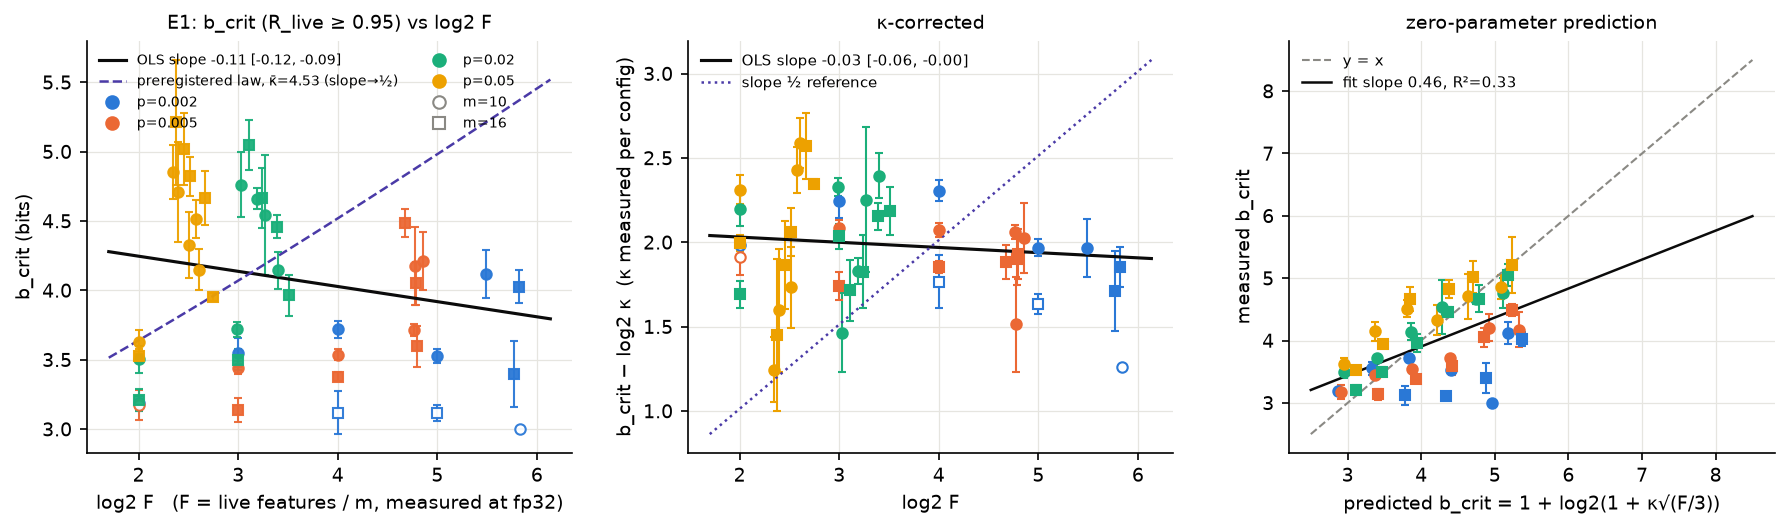
\includegraphics[width=\linewidth]{fig1_bcrit_vs_F_R_live_95.png}
\caption{\textbf{Money plot, negative.} Critical bit-width (RTN, QAT, retention $R_{\mathrm{live}}=0.95$) against
$\log_2 F$ for the E1 grid ($m\in\{10,16\}$, four $p$, mean $\pm$ SD over 4 seeds). Left: OLS slope %E1SLOPE% bits per
doubling (bootstrap CI %E1CI%) against the preregistered $\nicefrac12$ (dashed: Eq.~\ref{eq:law} with the mean measured
$\kappa$). Middle: $\kappa$-corrected. Right: the zero-parameter prediction of Eq.~\ref{eq:law} against measurement.}
\label{fig:money}
\end{figure}
Figure~\ref{fig:money} is the preregistered test. Over %NCFG% configurations spanning $F = %FMIN%$ to $%FMAX%$ (measured live
columns per dimension; $\kappa$ from $%KMIN%$ to $%KMAX%$), $b_{\mathrm{crit}}$ is %BRANGE% bits and its slope in $\log_2 F$ is
%E1SLOPE% [%E1CI%]---in the preregistered ``hypothesis dead'' band ($<0.15$), and the CI excludes $\nicefrac12$ by a wide
margin. The result is threshold-robust (90\,\%: %E1SLOPE90%; 99\,\%: %E1SLOPE99%), holds on the continuous axis built from the
measured residual $\hat\sigma_\varepsilon$ (%E1SLOPEBEFF%), and holds for the preregistered hard count where it is defined
(%E1SLOPEHARD%). Applying the same quantizer post-training to the converged fp32 models (E3) gives the same answer with
smaller error bars: RTN $b_{\mathrm{crit}} = %PTQRANGE%$ across all cells, slope %PTQSLOPE%; per-channel scaling lowers
it uniformly to %PCRANGE%. Quantization-aware training buys essentially nothing over post-training rounding at this
threshold (%QATVSPTQ%).

\subsection{What sets the threshold: a universal perturbation tolerance and the outlier ratio (E3)}
\begin{figure}[t]
\centering
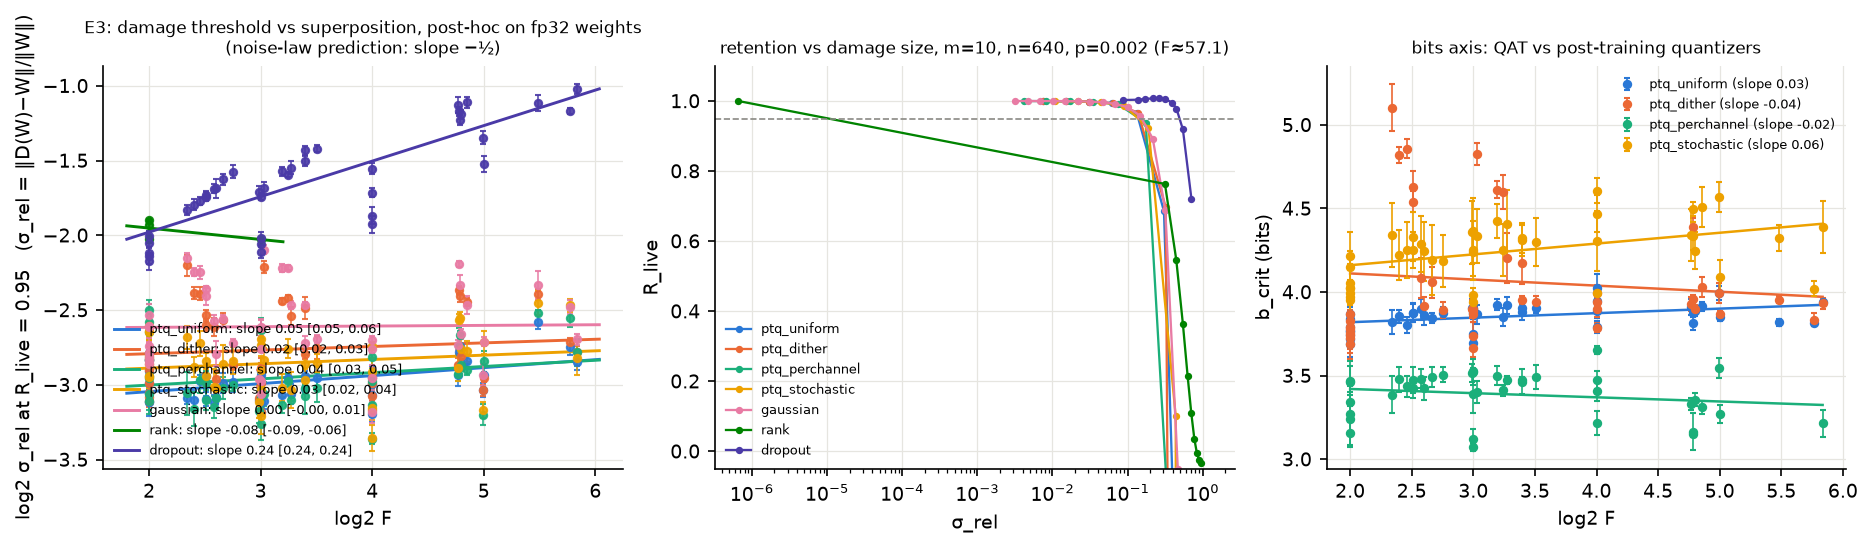
\includegraphics[width=\linewidth]{fig3_anydamage_null.png}
\caption{\textbf{Any-damage null (post-hoc on the E1 fp32 checkpoints).} Left: relative perturbation at which the
represented features lose 5\,\% of their explained variance, $\sigma_{\mathrm{rel,crit}}$, against $\log_2 F$ for seven damage
families; the preregistered noise-floor prediction was slope $-\nicefrac12$. Middle: $R_{\mathrm{live}}$ against
$\sigma_{\mathrm{rel}}$ for one configuration---the noise-like families collapse onto one curve. Right: bit-width axis,
QAT vs post-training quantizers.}
\label{fig:e3}
\end{figure}
Figure~\ref{fig:e3} shows why. Every noise-like damage family---RTN, per-channel RTN, dithered and stochastic rounding,
Gaussian noise---crosses the 5\,\% line at a relative perturbation $\sigma_{\mathrm{rel,crit}} \approx %SIGRANGE%$ that is flat in
$F$ (slopes %E3SLOPES%; predicted $-\nicefrac12$), and their retention curves collapse when plotted against
$\sigma_{\mathrm{rel}}$. Structured damage behaves differently: feature dropout is tolerated up to
$\sigma_{\mathrm{rel}}\approx%DROPRANGE%$ because removing a marginal feature also removes the interference it caused, and rank
truncation is catastrophic at any level (removing one of $m$ directions already costs $>5\,\%$). The bit-width then follows
from the quantizer's residual alone. With the measured $\kappa_{\mathrm{live}}$ ($%KLRANGE%$) and the measured
$\sigma_{\mathrm{rel,crit}}$ of RTN, Eq.~\eqref{eq:corrected} predicts $b_{\mathrm{crit}}$ to within %CORRERR% bits with no
fitted parameter (pilot: predicted 3.68/3.61/3.82/3.85 vs measured 3.84/3.81/3.83/3.85 for $F = 56/25/8.6/5.2$).
Dithered quantization is \emph{worse} than the shared lattice by 0.2--1.5 bits, and increasingly so at low live fraction:
dither moves the exact zeros of the dead columns off the lattice and wakes them as interferers. A lattice that contains
$0$ is what makes rounding benign for sparse weight matrices.

\subsection{Translation vs tilt (E4) and importance ordering (E5)}
%E4E5%

\subsection{Moving $\kappa$ at fixed $F$ (E6)}
%E6%

\subsection{GPT-2 small: outliers, not superposition, predict per-matrix quantization sensitivity}
\begin{figure}[t]
\centering
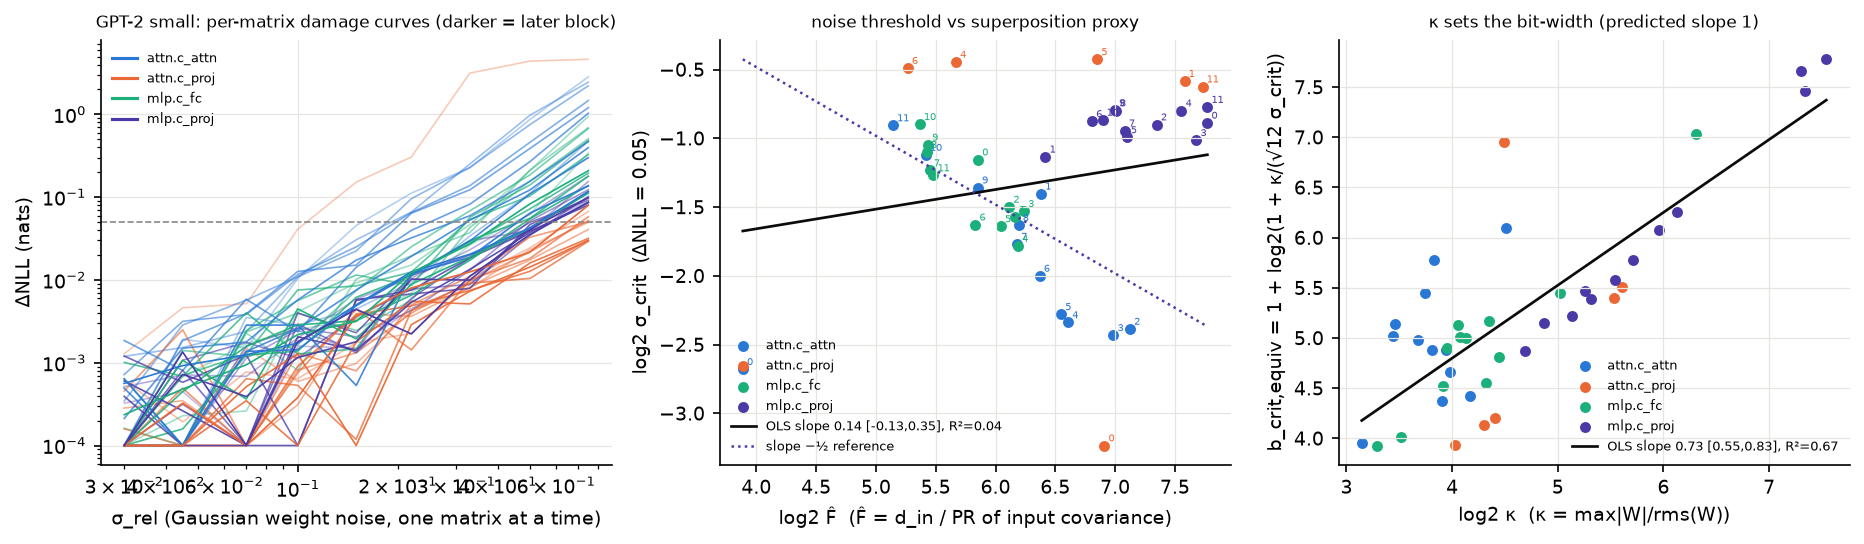
\includegraphics[width=\linewidth]{fig7_lm_layers.png}
\caption{\textbf{GPT-2 small, 48 weight matrices, one damaged at a time.} Left: $\Delta$NLL against relative Gaussian
weight noise (darker = later block). Middle: noise threshold ($\Delta\mathrm{NLL}=0.05$) against the superposition proxy
$\hat F = d_{\mathrm{in}}/\mathrm{PR}$; preregistered slope $-\nicefrac12$ dotted. Right: the bit-width equivalent of the noise
threshold against $\log_2\kappa$.}
\label{fig:lm}
\end{figure}
The per-matrix noise threshold carries no information about the superposition proxy: slope $+0.14$ [$-0.13$, $0.35$],
$R^2=0.04$ at $\Delta\mathrm{NLL}=0.05$ (and $R^2 \le 0.03$ at $0.02$ and $0.10$). The outlier ratio does carry it. The
independently measured per-tensor RTN cliff of each matrix follows $\log_2\kappa$ with slope $0.63$ [$0.49$, $0.76$],
$R^2=0.53$ ($n=34$ uncensored), against $0.28$ [$-0.02$, $0.61$], $R^2=0.14$ for $\log_2\hat F$; in a joint fit
$b_{\mathrm{crit}} = 2.40 + 0.72\log_2\kappa - 0.12\log_2\hat F$. Converting each matrix's noise threshold to a bit-width with
Eq.~\eqref{eq:corrected} reproduces its measured RTN cliff with slope $0.92$, $R^2=0.68$ and a mean error of $-0.23$ bits.
Two refinements matter in practice. First, the $\kappa$ slope is $0.6$--$0.7$ rather than $1$ because outlier-heavy matrices
also tolerate more relative noise ($\sigma_{\mathrm{crit}}\propto\kappa^{0.46}$): their energy sits in a few entries, so a
unit of relative perturbation moves the directions that matter less. Second, per-tensor RTN on the three
$\kappa\approx160$--$190$ matrices (mlp.c\_proj of blocks 1--3) is pathological---everything but the outliers rounds to
zero at every width $\le 6$, damage is non-monotone in bits, and joint damage is $3\times$ super-additive (all 48 matrices at 6
bits: $+4.6$ nats vs.\ $1.6$ summed)---which is precisely the regime the toy analysis flags as ``$q_{\max}\Delta$ larger than the
bulk''. With per-channel scaling this regime disappears, and the relevant statistic becomes the norm-weighted per-channel
outlier ratio $\kappa_{\mathrm{eff}}$: %PCRESULT%.

\subsection{A calibration-free bit allocator}
%MIXED%


\section{Discussion and limitations}
%DISCUSSION%


\begin{thebibliography}{9}
\bibitem{elhage2022toy} N.~Elhage, T.~Hume, C.~Olsson, N.~Schiefer, T.~Henighan, S.~Kravec, Z.~Hatfield-Dodds, R.~Lasenby, D.~Drain, C.~Chen, R.~Grosse, S.~McCandlish, J.~Kaplan, D.~Amodei, M.~Wattenberg, C.~Olah. Toy models of superposition. \emph{Transformer Circuits Thread}, 2022.
\bibitem{hooker2019} S.~Hooker, A.~Courville, G.~Clark, Y.~Dauphin, A.~Frome. What do compressed deep neural networks forget? arXiv:1911.05248, 2019.
\bibitem{hooker2020} S.~Hooker, N.~Moorosi, G.~Clark, S.~Bengio, E.~Denton. Characterising bias in compressed models. arXiv:2010.03058, 2020.
\bibitem{dettmers2022} T.~Dettmers, M.~Lewis, Y.~Belkada, L.~Zettlemoyer. LLM.int8(): 8-bit matrix multiplication for transformers at scale. \emph{NeurIPS}, 2022.
\bibitem{xiao2023} G.~Xiao, J.~Lin, M.~Seznec, H.~Wu, J.~Demouth, S.~Han. SmoothQuant: accurate and efficient post-training quantization for large language models. \emph{ICML}, 2023.
\bibitem{lin2024awq} J.~Lin, J.~Tang, H.~Tang, S.~Yang, W.-M.~Chen, W.-C.~Wang, G.~Xiao, X.~Dang, C.~Gan, S.~Han. AWQ: activation-aware weight quantization for LLM compression and acceleration. \emph{MLSys}, 2024.
\bibitem{frantar2022gptq} E.~Frantar, S.~Ashkboos, T.~Hoefler, D.~Alistarh. GPTQ: accurate post-training quantization for generative pre-trained transformers. arXiv:2210.17323, 2022.
\bibitem{inputs2025} Why do some inputs break low-bit LLM quantization? arXiv:2506.12044, 2025.
\bibitem{bitnets} Toy models of superposition: what about BitNets? \emph{LessWrong}, 2024.
\end{thebibliography}

\appendix
\section{Appendix}
%APPENDIX%

\end{document}
